\documentclass[a4paper]{article}

\usepackage[english]{babel}
\usepackage[utf8]{inputenc}
\usepackage{amsmath}
\usepackage{graphicx}
\usepackage{listings}
\usepackage[parfill]{parskip}
\usepackage[colorinlistoftodos]{todonotes}
\usepackage[colorlinks=true,urlcolor=blue,linkcolor=blue]{hyperref}

\title{University of Kansas High School Design Programming: Rules, Resources, and Examples}

\date{November 5, 2014}

\author{Engineering SELF Fellows, Association for Computing Machinery}

\begin{document}
\lstset{
    language=java,
    basicstyle=\ttfamily,
    numbers=left,
    numbersep=8pt,
    showspaces=false,
    showstringspaces=false
}
\maketitle

\tableofcontents

\newpage

\section{Introduction}

Welcome to the High School Design Programming Competition! This competition has been designed to test your knowledge of programming as a tool for general problem solving in your choice of the following languages:
\begin{center}
    C \\
    C\texttt{++} \\
    Java \\ 
    Python (v. 2.6 and 3.4) \\
    Ruby \\
\end{center}

\newpage

\section{Rules}

You will be given a docket describing a total of 10 programming challenges, arranged in ascending difficulty, and you will be allotted three and a half hours, in a single block of time, to write solution programs for these challenges. An automated system called DOMJudge provides a website interface where you can submit your solutions for judging, receive feedback, and check a running scoreboard and clock. 

All problems will be described in a uniform fashion: An introduction to the problem will set up the scenario and describe what challenge you must write a program to solve. It will then describe how the input your program must read will be structured, and it will prescribe how the program's output must be formatted in order to be read correctly. An example of input and output will be provided for you to check your program against. \textbf{Note}: when your program is actually judged, different input data will be used, but the formatting will be the same. 

Each correct problem is worth 1 point, so whichever team completes the most problems out of 10 will be designated the winner. In the case of ties, time (as marked in seconds, running from the beginning of the competition) will be used as a tiebreaker. So if more than 1 team completes all 10 problems, the first team to have done so is the winner. You may submit your solutions for judging as many times as you need to, but you should be aware that each time you submit a solution that is judged to be incorrect, you will receive a time penalty that will add to your total time, so it is best to work hard to ensure your program is correct before submitting for judging. However, even if your submission turns out to be wrong, you should feel free to rework it until you get it right or decide to move on to another problem. 

Teams may consist of up to two students. You will not be allowed use of the Internet except for access to the DOMJudge web interface, but any books on your programming language may be used. 

\newpage

\section{Concepts}

In this section, we list the core programming concepts you should be familiar with in your langauge(s) of choice. All the problems day-of the competition will be solvable using just the concepts mentioned here. However, as the problems get more difficult, solutions will take less time to draft, code, and test if your team is well practiced and quite familiar with your chosen languages. Although we list here the basic concepts necessary to compete, we encourage you to read more in depth about features of your language, so that you may be more creative and efficient in writing your solutions. You may already be familiar with the basic stuff. If so, treat what follows as a refresher, then get to practice! In our little example snippets below, the code is Java.

\subsection{Assignment and Arithmetic}
All languages have some manner of giving names to data and doing basic operations on that data. You should be familiar with how your language declares variables and assigns values to them. You should also know how your language performs arithmetic operations, like addition and multiplication. In particular, you will want to be familiar with `Modular Arithmetic', an operation that works by finding the remainder when you divide one integer number by another. Other useful math functions are Ceiling and Floor, which round decimals up or down to the nearest integer.

You should also know about all the different `primitive' data types your language has. Most languages can natively represent strings of characters, single characters, Boolean values (true and false), integers, and decimal numbers. But for some languages, 3 / 4 may not be the same as 3 / 4.0. Knowing little quarks about your language keeps you from running into odd errors.

\subsection{Conditionals}
Conditional branches allow you to evaluate logic -- in particular, they allow your program to change the instructions it will execute depending on the kind of data your program was given. The most common way to represent conditional choice in a program is with \texttt{if else} statements. In general, when your program reaches a conditional block of code, it determines whether or not the condition following the \texttt{if} is true. For example:

\begin{lstlisting}
int x = 4;
if (x == 5) {
    System.out.println("x is five!");
} else {
    System.out.println("x is not five, bummer");
}
\end{lstlisting}

Here, we let our integer x be 4. When we reach our conditional, we check if x equals 5. If it does, we'd print out ``\textit{x is five!}'', but in our case, x does not equal 5, so instead we would evaluate the \texttt{else} portion and print ``\textit{x is not five, bummer}''. Most languages will also let you chain several \texttt{if else} statements together,

\begin{lstlisting}
String ourSentence = "Coi ro do!";
if (ourSentence.equals("Hi there!")) {
    System.out.println("Hi right back at ya!");
} else if (ourSentence.equals("I have to go..")) {
    System.out.println("See ya later!");
} else {
    System.out.println("Sorry, I don't speak Lojban!");
}
\end{lstlisting}

Above, we use Java's special \texttt{equals} method to check if a string is the same as another string. So there are lots of things that can be used to create a conditional statment in an \texttt{if else} block. And on top of that, you can put together several conditionals using logical operators \texttt{\textbar\textbar} for \textit{or} and \texttt{\&\&} for \textit{and}. For example, \texttt{if (x * 2 == 4)\textbar\textbar (x >= 10)} reads as \textit{if x times 2 is equal to four or, if x is greater than or equal to 10...}. 

So for conditionals, you should know how your language writes \texttt{if else} blocks, what methods or operations can check if something is \textit{true} or \textit{false}, and how conditionals can be linked together using \textit{and} and \textit{or}.

\subsection{Loops}
Loops let you repeat a block of code again and again either a certain number of times, or until some condition (remember those?) is met. The basic loops for Java, C, and C\texttt{++} are \texttt{for}, \texttt{while}, and \texttt{do while}. Python and Ruby have loops named the same, but they look and work slightly different. Review for your language what loops you have and how they work.

\subsection{Data Structures}
When we say \textit{Data Structures}, we really just mean containers. Common containers in Java, C, and C\texttt{++} include Arrays, Lists (or Vectors), and Hashmaps. Arrays and Lists are the simplest. Arrays are like a line of cubby holes, they have fixed length, and can be filled up with only one type of data at a time, like an \textit{Array of integers} or an \textit{Array of Strings}. Lists work similarly, but can grow in length. Both of these structures let you check what value was assigned to a particular index, and they let you assign values to indices. Hashmaps (also sometimes called Dictionaries) let you give pair a value to a keyword so that you can look up values if you know their keywords, or you can check if a value is in the hashmap. Arrays, Lists, and Hashmaps all have different ways of being used, and are useful at different times. You should be familiar with what Data Structures your language has and the ways they can be used. Arrays and Lists though will be your bread and butter for most problems at the competition.

\textbf{Note:} In Python and Ruby, Lists are usually preferred to Arrays for the sake of simplicity. 

\subsection{Functions and Methods}
All languages have special commands that either return specific pieces of information, or transform data in some way. For example, in Java, if we want to know the length of a string in the variable \texttt{ourString}, we could use \texttt{int stringLength = ourString.length();}, which would give an integer representing the length of the string. In Python, if we wanted to know the size of a list \texttt{ourList}, we could use \texttt{listLength = len(ourList)}. All the methods and functions of a language are described by the language's \textit{Standard Library}. The list of total methods and functions in the Standard Library is often quite large, but it'll be fine if you just get familiar with those related to your language's data structures and Strings. 

Most languages will also let you define your own methods and functions elsewhere inside your program. This can help your code keep clean if you find yourself repeating some pattern of operations multiple times, and knowing how your language declares and uses them may be helpful.

\subsection{Going Forward}
To best learn and practice the concepts listed above, we recommend you check out the websites \url{http://www.codecademy.com} or \url{http://www.codingbat.com}. They'll give you lots of simple challenges and tutorials that will introduce you to the languages supported by the competition. Each of them have lots of examples and even videos to help you learn the basic concepts in writing programs.

\section{DOMJudge}
\subsection{Summary}
Here we include a short summary of the DOMJudge system interface, the web-portal by which you will submit your solutions for automated judging. The single constraint of this system is that your programs \textbf{must} be written to accept their input from \texttt{stdin} and write their output to \texttt{stdout} (also sometimes referred to as \textit{writing to the console}). We talk a little more about what this means in the examples portion of this section. What follows is an introduction to the interface.

\subsection{Interface}
A web URL will be provided to you from which you will gain access to the DOMJudge submission interface. From your team pagei, \url{http://example.com/domjudge/team}, you will select \textbf{Select file...} in the left column and select the file of your source code to submit. By default, the problem is selected from the base of the filename and the language from the your file's file extension. 

Viewing scores, submissions, and sending and reading clarification requests is done through the web team interface, \url{http://example.com/domjudge/team}. 

\begin{figure}[p]
    \centering
    \fbox{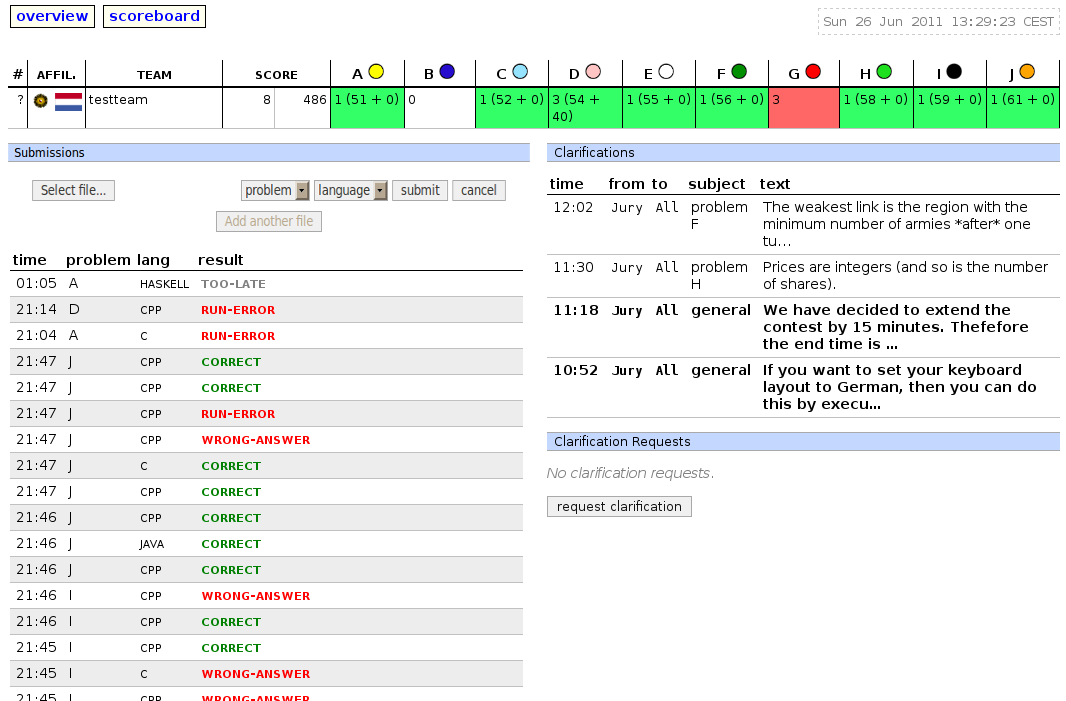
\includegraphics[width=14cm]{team-overview.png}}
    \caption{the web team interface overview page}
    \label{fig:team-overview}
\end{figure}

\begin{figure}[p]
    \centering
    \fbox{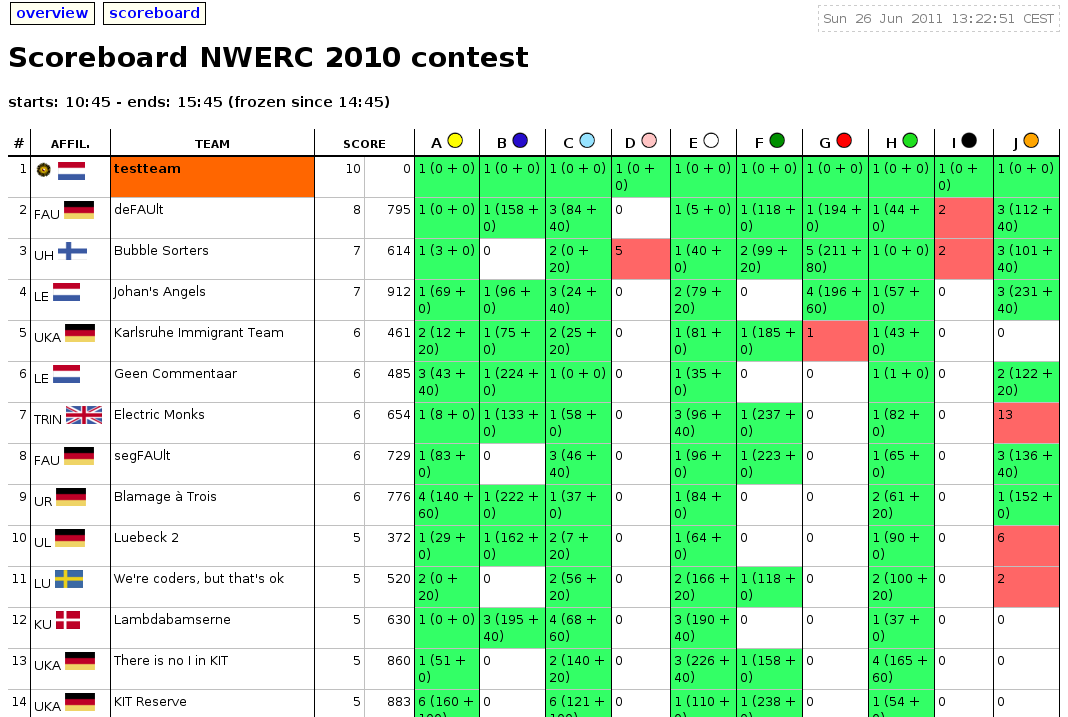
\includegraphics[width=14cm]{team-scoreboard.png}}
    \caption{the scoreboard webpage}
    \label{fig:team-scoreboard}
\end{figure}

The left column of the team interface shows your teams's row in the scoreboard: your position and the which problems you attempted and which you solved. Via th menu, you can view the public scoreboard page with scores of all the teams. The score column lists the number of problems solved and the total penalty time. Each cell in the problem column lists the number of submissions, and if th problem was solved as well as the time of the first correct submission for that problem since the contest start. Submissions can have the following resuts:

\begin{description}
    \item[CORRECT:]
        The submission passed all tests: you solved this problem!

    \item[COMPILER-ERROR:]
        There was an error when compiling your program. On the submission
        details page you can inspect the exact error (this option might be
        disabled).

    \item[TIMELIMIT:]
        Your program took longer than the maximum allowed time for this
        problem. Therefore it has been aborted. This might indicate that your
        program hangs in a loop or that your solution is not efficient
        enough.

    \item[RUN-ERROR:]
        There was an error during the execution of your program. This can have
        a lot of different causes like division by zero, incorrectly
        addressing memory (e.g. by indexing arrays out of bounds), trying to
        use more memory than the limit, etc.
        Also check that your program exits with exit code 0!

    \item[NO-OUTPUT:]
        Your program did not generate any output. Check that you write to
        standard out.

    \item[WRONG-ANSWER:]
        The output of your program was incorrect. This can happen simply
        because your solution is not correct, but remember that your output
        must comply exactly with the specifications of the jury.

    \item[PRESENTATION-ERROR:]
        The output of your program has differences in presentation with the
        correct results (for example in the amount of whitespace). This will,
        like WRONG-ANSWER, count as an incorrect submission. This result is
        optional and might be disabled.

    \item[TOO-LATE:]
        Bummer, you submitted after the contest ended! Your submission is
        stored but will not be processed anymore.
\end{description}

You are allowed to communicate with the jury, we omniscient few who oversee the entirety of the competition namelessly, and behind the inscrutability of teletype terminals, through the use of clarifications. These can be found in the right column of your team page. Both clarification replies from the jury and requests sent by your are displayed there. 

There is also a button to submit a new clarification request to the jurry. This request is only readable for the jury and they will respond as soon as possible. If the jury deems an answer relevant to everyone, it will be viewable to everyone. 

\subsection{Testing}
The DOMJudge system is fully automated. Once input/output files have been prepared to verify your program, no other human element is necessary in scoring besides clarifications on the part of the jury. But this is how it works:

With the web interface you can submit the source code of your solution to the jury. Note that you must send your source code, not a compiled version of the program. Your solution is then sent over the network to a judging computer that will automatically compile or interpret your solution and pipe the proper input file to the program. The output of your program will then be compared against the validated output file. If your output matches the expected output, your program is correct. If not, you will receive some information about what went wrong before you go back to the drawing board. 

\subsection{Examples of Proper Input/Output}
Here we define how you must write your program to read from \texttt{stdin} and write to \texttt{stdout} for the languages supported by this competition. We do this through annotation of an example program.

\textbf{Description:} Write a program to send a friendly greeting! 

\textbf{Input:} The first line will be an integer representing the number of lines to read. Each subsequent line will be a single name.

\textbf{Output:} On a new line for each, print out the name you read as part of the string ``Hello \textless name\textgreater!''.

\textbf{Sample:}

\begin{tabular}{|p{0.47\textwidth}|p{0.47\textwidth}|}
    \hline
    \textbf{input} & \textbf{outout} \\
    \hline
    \begin{verbatim}
    3
    World
    Alan
    Ada
    \end{verbatim} &
    \begin{verbatim}
    Hello world!
    Hello Alan!
    Hello Ada!
    \end{verbatim} \\
    \hline
\end{tabular}
\newpage

A solution for the problem in C:
\begin{lstlisting}[language=C]
#include <stdio.h>

int main() {
    int ntests;
    char name[100]

    scanf("%d\n", &ntests);

    int i;
    for (i = 0; i < ntests; i++) {
        scanf("%s\n", name);
        printf("Hello %s\n", name);
    }

    return 0;
}
\end{lstlisting}

Here, we note that C uses the \texttt{scanf} function to read from \texttt{stdin} and \texttt{printf} to write to \texttt{stdout}. It declares an integer variable \texttt{ntests}, and \texttt{scanf} reads in a value from the console and assigns that to \texttt{ntests} (we note that \texttt{scanf} really uses a \textit{reference} to \texttt{ntests}, that's what the \textit{and} sign means, but that's special C stuff). \texttt{scanf} is later used with a character array that will hold our names. Our character array's size is 100, which is just arbitrarily large so we can hold any name we might read. We then use the \texttt{printf} function to print out our strings to \texttt{stdout} as we loop through them. We have to always \texttt{return 0} or else our program will \textbf{error}! 

A solution in C\texttt{++}:
\begin{lstlisting}[language=C++]
#include <iostream>
#include <string>

using namspace std;

int main() {
    int ntests;
    string name;

    cin >> ntests;
    for (int i = 0; i < ntests; i++) {
        cin >> name;
        cout << "Hello " << name << "!" << endl;
    }

    return 0;
}
\end{lstlisting}

C\texttt{++} uses \texttt{cin >>} to push \texttt{stdin} lines into a variable on the right, and uses \texttt{cout >>} to print out lines from the right to \texttt{stdout}. C\texttt{++} also has real strings, not just character arrays. Other than that, the logic of this solution is the same as the solution in C.

A solution in Java:
\begin{lstlisting}[language=Java]
import java.io.*;

class Main {
    public static BufferedReader in;

    public static void main(String[] args) throws IOException {
        in = new BufferedReader(new InputStreamReader(System.in));

        int nTests = Integer.parseInt(in.readline());

        for (int i = 0; i < nTests; i++) {
            String name = in.readLine();
            System.out.println("Hello " + name + "!");
        }
    }
}
\end{lstlisting}

For Java, we first note our class \textbf{needs} to be named \textit{Main}. Java uses a \texttt{BufferedReader} object that it imports from \texttt{java.io.*}, which it uses to gather input from \texttt{System.in}. Using the command \texttt{System.out.println(...)} will let you write to \texttt{stdout}.

A solution in Pythoni 2.7:
\begin{lstlisting}[language=Python]
import fileinput
import sys

num = sys.stdin.readline()

for line in fileinput.input():
    print "Hello " + line.strip() + "!"
\end{lstlisting}

For Python 2.7, we import \texttt{fileinput} and \texttt{sys} to get our input from \texttt{stdin}. Python has some looping mechanisms that will allow us to cleverly not need the integer representing the number of lines, the command on line 4 reads it in, but does nothing with it. The special Python \texttt{for} loop on line 6 will loop over all the lines from \texttt{stdin} and store each one temporarily in the variable \texttt{line}. It's worth noting that if we read in the lines this way, we need to strip off the hidden \texttt{newline} character that separates each line of input from the string we've read in. \texttt{strip()} does that for us. Then we just print it out to \texttt{stdout} with the aptly named \texttt{print} function.
\newpage

A solution in Python 3:
\begin{lstlisting}[language=Python]
import fileinput
import sys

num = sys.stdin.readline()

for line in fileinput.input():
    print("Hello " + line.strip() + "!")
\end{lstlisting}
Python comes in two common versions. Python 2.7 and Python 3 are just different enough that it matters. All we notice here is that the Python 3 \texttt{print} command wraps its contents in parenthesis. There are some other differences too, so make sure you know which version of Python you're using. 

\textbf{Note:} for both versions of Python, it's common to include \textit{interpreter directives} at the top of the file, that may look like \texttt{\#!/usr/bin/python}. You must \textbf{not} include a line like this in your submission. DOMJudge will be mad at you. If this doesn't look familiar to you anyway, just forget about it and go on with your life. 

A solution in Ruby:
\begin{lstlisting}[language=Ruby]
$stdin.each_line.each_with_index do |line, i|
    if i == 0
        next
    end
    puts "Hello #{line.strip}!"
end
\end{lstlisting}

Ruby uses a special variable \texttt{\$stdin} to represent console input. The method \texttt{each\_line} grabs all the lines from \texttt{stdin} at one time, and the method \texttt{each\_with\_index} allow us to keep track of our position in the loop. Since the first line is just a silly integer, we can use the index of 0 to skip it, then we can do what we'd like with subsequent lines. In our case, we use the function \texttt{puts} to write to \texttt{stdout}. You'd likely replicate this looping pattern if you decide to use Ruby.

\subsection{Going Forward}
Now that you know how DOMJudge expects you to use Input/Output, feel free to log into the guest account of our test DOMJudge instance and review the practice problems there. You can also get a feel for the environment you'll use to judge submit your programs. Additional practice problems and even examples of solutions can be found at the github repository of the KU chapter of the Assocation for Computing Machinary, \url{https://github.com/KU-Competitive-Programming/Weekly-Problems}. Here we keep a backlog of interesting challenges and solutions our members have submittted in the past. Any problem headed \textit{Beginner} should be good for you to read the description of. 

\end{document}
